\documentclass[14pt]{extbook}
\usepackage{multicol, enumerate, enumitem, hyperref, color, soul, setspace, parskip, fancyhdr} %General Packages
\usepackage{amssymb, amsthm, amsmath, bbm, latexsym, units, mathtools} %Math Packages
\everymath{\displaystyle} %All math in Display Style
% Packages with additional options
\usepackage[headsep=0.5cm,headheight=12pt, left=1 in,right= 1 in,top= 1 in,bottom= 1 in]{geometry}
\usepackage[usenames,dvipsnames]{xcolor}
\usepackage{dashrule}  % Package to use the command below to create lines between items
\newcommand{\litem}[1]{\item#1\hspace*{-1cm}\rule{\textwidth}{0.4pt}}
\pagestyle{fancy}
\lhead{Progress Quiz 8}
\chead{}
\rhead{Version B}
\lfoot{4553-3922}
\cfoot{}
\rfoot{Fall 2020}
\begin{document}

\begin{enumerate}
\litem{
Solve the radical equation below. Then, choose the interval(s) that the solution(s) belongs to.\[ \sqrt{2 x - 5} - \sqrt{-4 x + 5} = 0 \]\begin{enumerate}[label=\Alph*.]
\item \( x \in [-0.07,0.45] \)
\item \( x \in [1.34,2.09] \)
\item \( \text{All solutions lead to invalid or complex values in the equation.} \)
\item \( x_1 \in [1.34, 2.09] \text{ and } x_2 \in [0.5,3.5] \)
\item \( x_1 \in [0.99, 1.39] \text{ and } x_2 \in [0.5,3.5] \)

\end{enumerate} }
\litem{
What is the domain of the function below?\[ f(x) = \sqrt[8]{9 x + 4} \]\begin{enumerate}[label=\Alph*.]
\item \( [a, \infty), \text{where } a \in [-3.25, -1.25] \)
\item \( (-\infty, \infty) \)
\item \( (-\infty, a], \text{where } a \in [-2.6, -1] \)
\item \( (-\infty, a], \text{where } a \in [-0.5, 0.2] \)
\item \( [a, \infty), \text{ where } a \in [-1.44, 0.56] \)

\end{enumerate} }
\litem{
Solve the radical equation below. Then, choose the interval(s) that the solution(s) belongs to.\[ \sqrt{6 x^2 + 54} - \sqrt{39 x} = 0 \]\begin{enumerate}[label=\Alph*.]
\item \( x_1 \in [-6, -2.5] \text{ and } x_2 \in [-5,0] \)
\item \( \text{All solutions lead to invalid or complex values in the equation.} \)
\item \( x_1 \in [-1, 3.9] \text{ and } x_2 \in [4.5,7.5] \)
\item \( x \in [-1,3.9] \)
\item \( x \in [3.7,6.6] \)

\end{enumerate} }
\litem{
Solve the radical equation below. Then, choose the interval(s) that the solution(s) belongs to.\[ \sqrt{-40 x^2 - 56} - \sqrt{96 x} = 0 \]\begin{enumerate}[label=\Alph*.]
\item \( x_1 \in [0.48, 2.13] \text{ and } x_2 \in [-0.6,1.8] \)
\item \( \text{All solutions lead to invalid or complex values in the equation.} \)
\item \( x_1 \in [-1.95, -1.21] \text{ and } x_2 \in [-1.8,0.6] \)
\item \( x \in [-1.15,-0.88] \)
\item \( x \in [-1.95,-1.21] \)

\end{enumerate} }
\litem{
Choose the graph of the equation below.\[ f(x) = - \sqrt[3]{x - 12} - 5 \]\begin{enumerate}[label=\Alph*.]
\begin{multicols}{2}\item 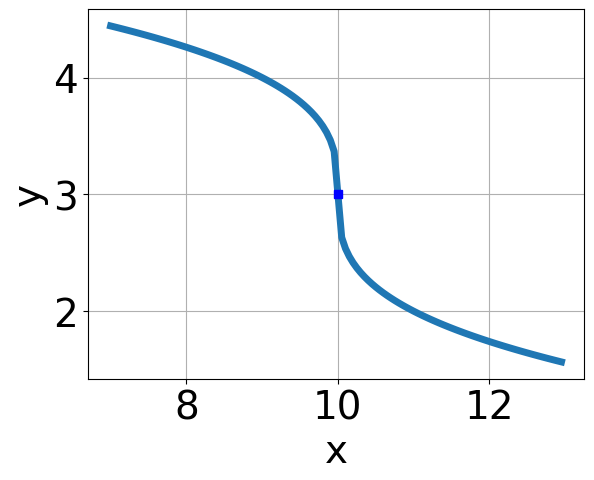
\includegraphics[width = 0.3\textwidth]{../Figures/radicalEquationToGraphAB.png}\item 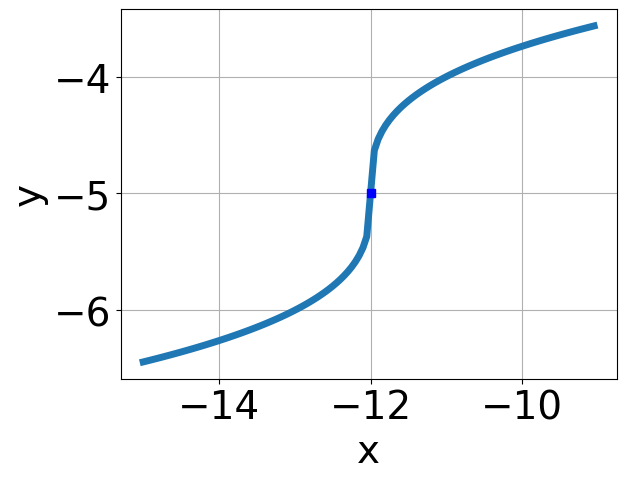
\includegraphics[width = 0.3\textwidth]{../Figures/radicalEquationToGraphBB.png}\item 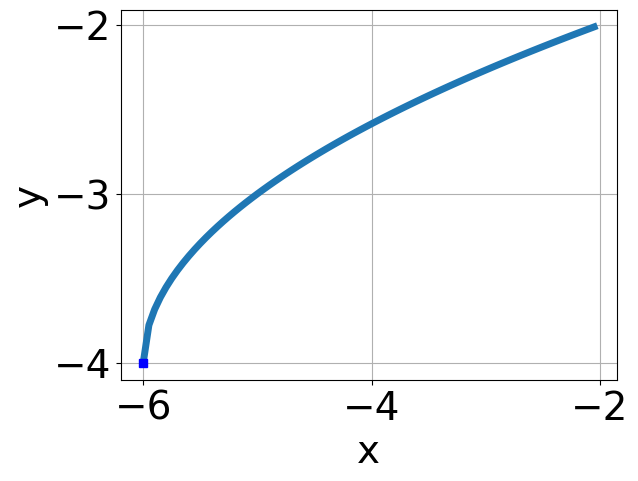
\includegraphics[width = 0.3\textwidth]{../Figures/radicalEquationToGraphCB.png}\item 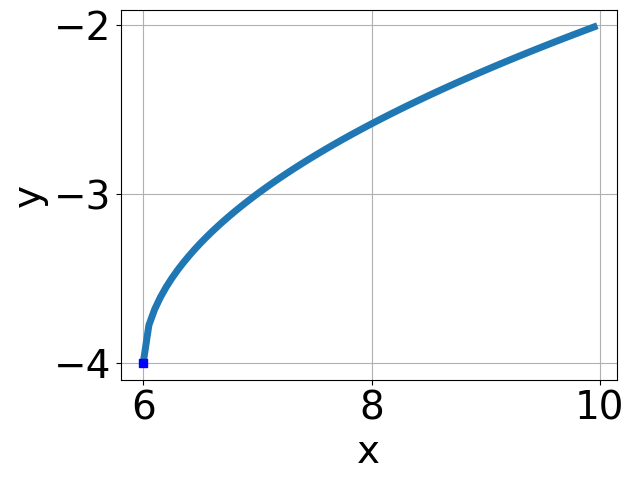
\includegraphics[width = 0.3\textwidth]{../Figures/radicalEquationToGraphDB.png}\end{multicols}\item None of the above.
\end{enumerate} }
\litem{
Choose the equation of the function graphed below.
\begin{center}
    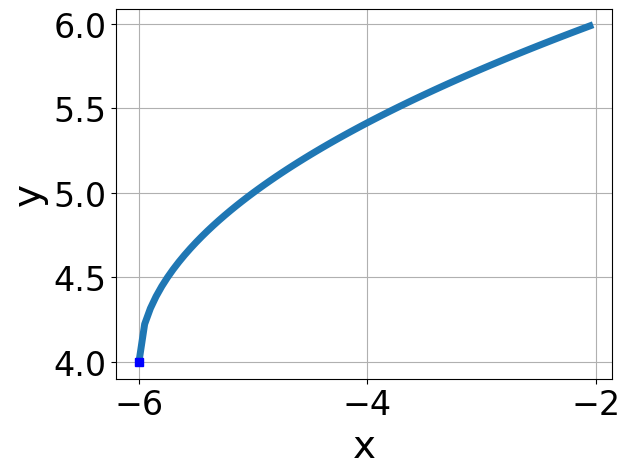
\includegraphics[width=0.5\textwidth]{../Figures/radicalGraphToEquationB.png}
\end{center}
\begin{enumerate}[label=\Alph*.]
\item \( f(x) = - \sqrt[3]{x + 14} - 7 \)
\item \( f(x) = \sqrt[3]{x - 14} - 7 \)
\item \( f(x) = - \sqrt[3]{x - 14} - 7 \)
\item \( f(x) = \sqrt[3]{x + 14} - 7 \)
\item \( \text{None of the above} \)

\end{enumerate} }
\litem{
Solve the radical equation below. Then, choose the interval(s) that the solution(s) belongs to.\[ \sqrt{-6 x - 9} - \sqrt{2 x - 6} = 0 \]\begin{enumerate}[label=\Alph*.]
\item \( x \in [-2.15,-1.6] \)
\item \( x_1 \in [-1.71, -1.42] \text{ and } x_2 \in [0,6] \)
\item \( x \in [-0.42,-0.07] \)
\item \( \text{All solutions lead to invalid or complex values in the equation.} \)
\item \( x_1 \in [-1.71, -1.42] \text{ and } x_2 \in [-2.38,1.62] \)

\end{enumerate} }
\litem{
Choose the equation of the function graphed below.
\begin{center}
    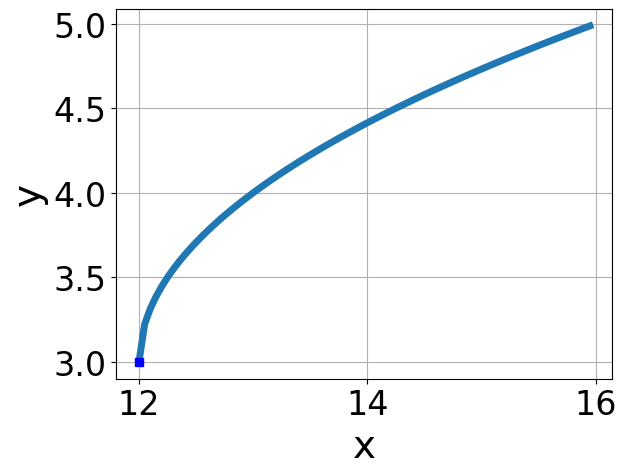
\includegraphics[width=0.5\textwidth]{../Figures/radicalGraphToEquationCopyB.png}
\end{center}
\begin{enumerate}[label=\Alph*.]
\item \( f(x) = \sqrt[3]{x + 14} - 5 \)
\item \( f(x) = - \sqrt[3]{x + 14} - 5 \)
\item \( f(x) = - \sqrt[3]{x - 14} - 5 \)
\item \( f(x) = \sqrt[3]{x - 14} - 5 \)
\item \( \text{None of the above} \)

\end{enumerate} }
\litem{
Choose the graph of the equation below.\[ f(x) = - \sqrt[3]{x - 14} + 7 \]\begin{enumerate}[label=\Alph*.]
\begin{multicols}{2}\item 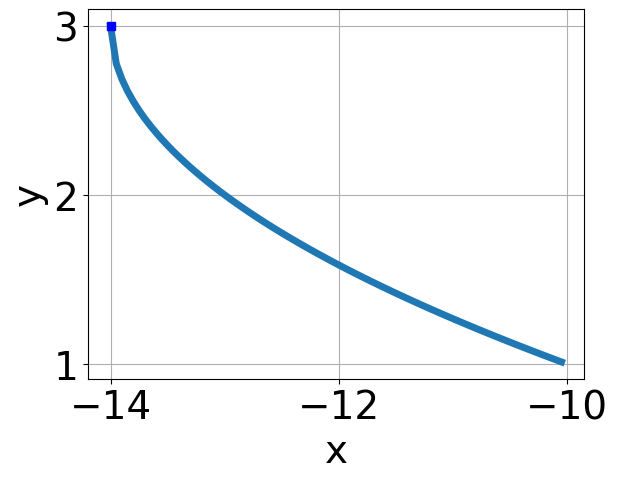
\includegraphics[width = 0.3\textwidth]{../Figures/radicalEquationToGraphCopyAB.png}\item 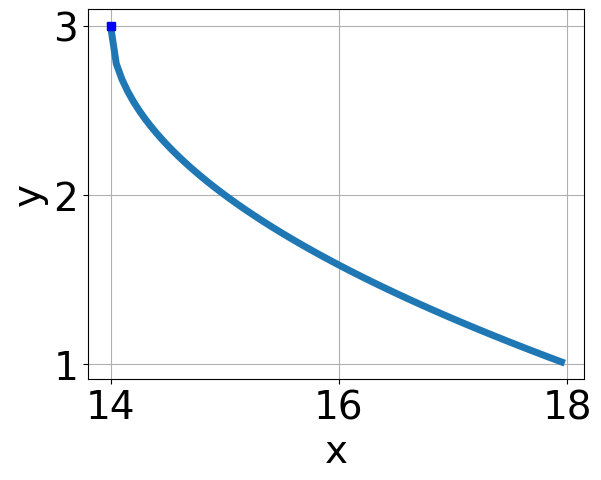
\includegraphics[width = 0.3\textwidth]{../Figures/radicalEquationToGraphCopyBB.png}\item 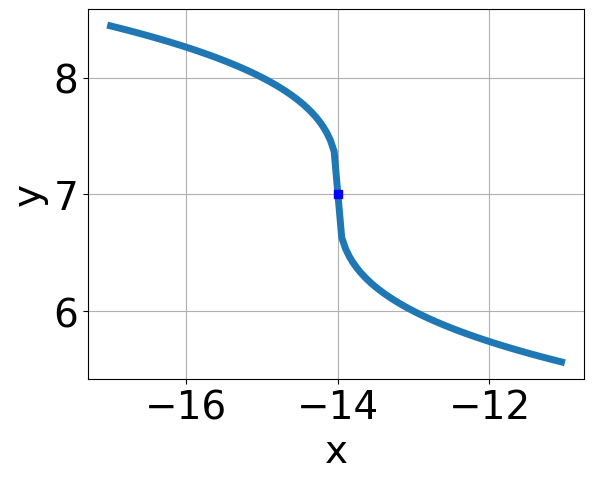
\includegraphics[width = 0.3\textwidth]{../Figures/radicalEquationToGraphCopyCB.png}\item 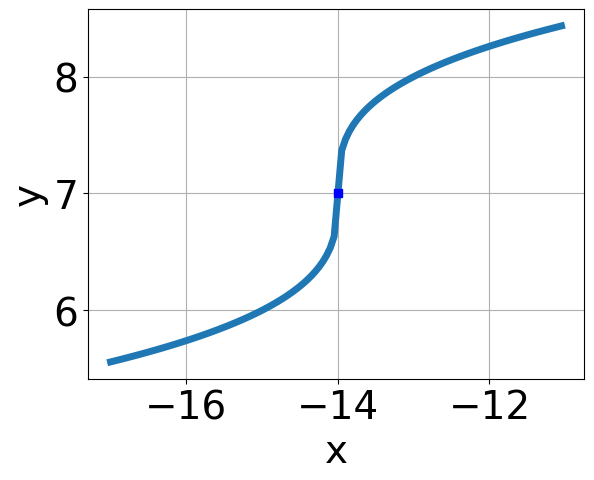
\includegraphics[width = 0.3\textwidth]{../Figures/radicalEquationToGraphCopyDB.png}\end{multicols}\item None of the above.
\end{enumerate} }
\litem{
What is the domain of the function below?\[ f(x) = \sqrt[4]{-3 x - 6} \]\begin{enumerate}[label=\Alph*.]
\item \( [a, \infty), \text{where } a \in [-1.4, 1.7] \)
\item \( [a, \infty), \text{where } a \in [-2.4, -1.1] \)
\item \( (-\infty, a], \text{where } a \in [-1.38, -0.14] \)
\item \( (-\infty, \infty) \)
\item \( (-\infty, a], \text{ where } a \in [-2.51, -1.82] \)

\end{enumerate} }
\end{enumerate}

\end{document}